\documentclass[a4paper,onecolumn]{article}
\usepackage{amsmath, amsthm, graphicx, amssymb, wrapfig, fullpage, subfigure, array,float}
\usepackage[]{algorithm2e}
\usepackage[toc, page]{appendix}
\usepackage{pdfpages, nomencl, pifont}
\usepackage[nottoc, numbib]{tocbibind}
\usepackage{tikz}
\usetikzlibrary{positioning,shadows,arrows}
\usepackage[font=sl, labelfont={sf}, margin=1cm]{caption}
\DeclareMathOperator{\e}{e}
\newtheorem{definition}{Definition}
\theoremstyle{remark}
\newtheorem{theorem}{Theorem}
\newtheorem{remarker}{Remark}
\makenomenclature

\begin{document}
\setcounter{page}{1}
\hspace{.36\textwidth}
\Large\textbf{Slides Outline}\\
\normalsize
\textbf{Research background}
\begin{enumerate}
    \item Motivation: 
          \begin{itemize}
              \item Optimization based on conservation law simulation. 
              \item Design space is high dimensional.
          \end{itemize}
          Example: optimization of turbulent return bend geometry. (picture)
    \item Many conservation law simulators are gray-box. What is gray-box / black-box / open-box. (table)
    \item Research scope:
          \begin{itemize}
              \item conservation law.
              \item gray-box simulation.
              \item high-dimension design.
          \end{itemize}
    \item Review of optimization methods : gradient-free, gradient-based.
    \item Challenges of both methods: 
          \begin{itemize}
              \item each simulation can be accurate but costly.
              \item if no adjoint, cost of gradient evaluation scales with dimension.
              \item grad-free can be costly. 
          \end{itemize}
    \item When lower-fidelity models are available, can save overall computation time by multi-fidelity optimization.
          \begin{itemize}
              \item Bayesian calibration / coKriging.
              \item Trust region.
          \end{itemize}
          High-fidelity model is the gray-box simulator; low-fidelity model can be constructed by surrogate methods.
    \item Review of surrogate methods. 
          \begin{itemize}
              \item physics-based surrogates: use the physics of the underlying system, such as
                    \begin{itemize}
                        \item coarser discretization: \emph{require simulator's PDE.}
                        \item reduced order model (POD, DEIM, balanced truncation): \emph{require simulator's PDE.}
                        \item simplified physics (RANS, dual porosity, thin airfoil theory).
                    \end{itemize}
              \item functional surrogate: use the sample value of objective function, such as
                    \begin{itemize}
                        \item radial basis function approximation.
                        \item polynomial approximation.
                        \item neural network.
                    \end{itemize}
          \end{itemize}
          Narrative: functional surrogate not suitable in my research scope because design space is high-dimensional. Focus on physics-based surrogate.
    \item Physics-based surrogates can be adaptive.
          \begin{itemize}
              \item Adaptive discretization: \emph{require simulator's PDE.}
              \item Goal oriented reduced order model: match observations, \emph{require simulator's PDE}
          \end{itemize}
\end{enumerate}

\newpage
\textbf{Twin model}
\begin{enumerate}
    \item Propose a adaptive physics-based surrogate that 
          \begin{itemize}
              \item does not require simulator's PDE, instead infer a PDE.
              \item PDE is inferred by matching the gray-box simulation's space-time solution.
          \end{itemize}
    \item Feasibility:
          Infer a general form PDE is not feasible, but we infer a conservation law.\\
          \begin{center}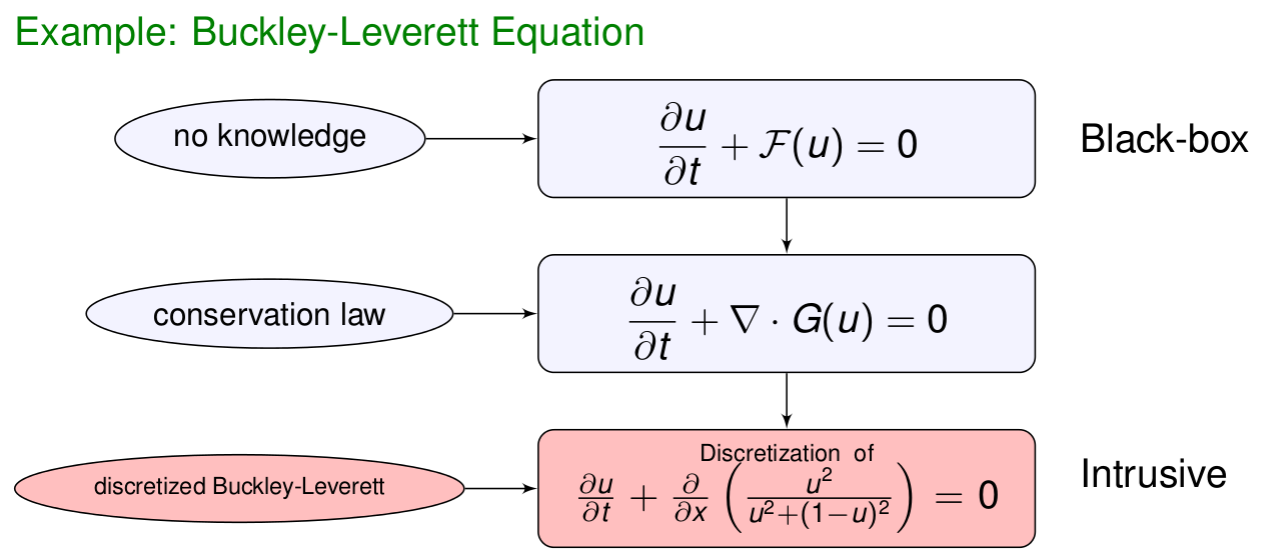
\includegraphics[width=4cm]{three_box.png}\end{center}
\end{enumerate}


\end{document}
